\documentclass[spec, och, referat]{shiza}
% параметр - тип обучения - одно из значений:
%    spec     - специальность
%    bachelor - бакалавриат (по умолчанию)
%    master   - магистратура
% параметр - форма обучения - одно из значений:
%    och   - очное (по умолчанию)
%    zaoch - заочное
% параметр - тип работы - одно из значений:
%    referat    - реферат
%    coursework - курсовая работа (по умолчанию)
%    diploma    - дипломная работа
%    pract      - отчет по практике
% параметр - включение шрифта
%    times    - включение шрифта Times New Roman (если установлен)
%               по умолчанию выключен
\usepackage{subfigure}
\usepackage{tikz,pgfplots}
\pgfplotsset{compat=1.5}
\usepackage{float}

%\usepackage{titlesec}
\setcounter{secnumdepth}{4}
%\titleformat{\paragraph}
%{\normalfont\normalsize}{\theparagraph}{1em}{}
%\titlespacing*{\paragraph}
%{35.5pt}{3.25ex plus 1ex minus .2ex}{1.5ex plus .2ex}

\titleformat{\paragraph}[block]
{\hspace{1.25cm}\normalfont}
{\theparagraph}{1ex}{}
\titlespacing{\paragraph}
{0cm}{2ex plus 1ex minus .2ex}{.4ex plus.2ex}

% --------------------------------------------------------------------------%


\usepackage[T2A]{fontenc}
\usepackage[utf8]{inputenc}
\usepackage{graphicx}
\graphicspath{ {./images/} }
\usepackage{tempora}

\usepackage[sort,compress]{cite}
\usepackage{amsmath}
\usepackage{amssymb}
\usepackage{amsthm}
\usepackage{fancyvrb}
\usepackage{listings}
\usepackage{listingsutf8}
\usepackage{longtable}
\usepackage{array}
\usepackage[english,russian]{babel}

% \usepackage[colorlinks=true]{hyperref}
\usepackage{url}

\usepackage{underscore}
\usepackage{setspace}
\usepackage{indentfirst} 
\usepackage{mathtools}
\usepackage{amsfonts}
\usepackage{enumitem}
\usepackage{tikz}
\usepackage{minted}

\newcommand{\eqdef}{\stackrel {\rm def}{=}}
\newcommand{\specialcell}[2][c]{%
\begin{tabular}[#1]{@{}c@{}}#2\end{tabular}}

\renewcommand\theFancyVerbLine{\small\arabic{FancyVerbLine}}

\newtheorem{lem}{Лемма}

\begin{document}

% Кафедра (в родительном падеже)
\chair{}

% Тема работы
\title{Диод Шоттки}

% Курс
\course{3}

% Группа
\group{331}

% Факультет (в родительном падеже) (по умолчанию "факультета КНиИТ")
\department{факультета КНиИТ}

% Специальность/направление код - наименование
%\napravlenie{09.03.04 "--- Программная инженерия}
%\napravlenie{010500 "--- Математическое обеспечение и администрирование информационных систем}
%\napravlenie{230100 "--- Информатика и вычислительная техника}
%\napravlenie{231000 "--- Программная инженерия}
\napravlenie{10.05.01 "--- Компьютерная безопасность}

% Для студентки. Для работы студента следующая команда не нужна.
% \studenttitle{Студентки}

% Фамилия, имя, отчество в родительном падеже
\author{Токарева Никиты Сергеевича}

% Заведующий кафедрой
% \chtitle{} % степень, звание
% \chname{}

%Научный руководитель (для реферата преподаватель проверяющий работу)
\satitle{аспирант} %должность, степень, звание
\saname{Р. А. Торгашов}

% Руководитель практики от организации (только для практики,
% для остальных типов работ не используется)
% \patitle{к.ф.-м.н.}
% \paname{С.~В.~Миронов}

% Семестр (только для практики, для остальных
% типов работ не используется)
%\term{8}

% Наименование практики (только для практики, для остальных
% типов работ не используется)
%\practtype{преддипломная}

% Продолжительность практики (количество недель) (только для практики,
% для остальных типов работ не используется)
%\duration{4}

% Даты начала и окончания практики (только для практики, для остальных
% типов работ не используется)
%\practStart{30.04.2019}
%\practFinish{27.05.2019}

% Год выполнения отчета
\date{2022}

\maketitle

% Включение нумерации рисунков, формул и таблиц по разделам
% (по умолчанию - нумерация сквозная)
% (допускается оба вида нумерации)
% \secNumbering

%-------------------------------------------------------------------------------------------
\tableofcontents

\intro

Диод -- электронный прибор с двумя (иногда тремя) электродами, обладающий односторонней проводимостью. Электрод, подключенный к положительному 
полюсу прибора, называют анодом, к отрицательному – катодом. Если к прибору приложено прямое напряжение, то он находится в открытом состоянии, 
при котором сопротивление мало, а ток протекает беспрепятственно. Если прикладывается обратное напряжение, прибор, благодаря высокому 
сопротивлению, является закрытым. Обратный ток присутствует, но он настолько мал, что условно принимается равным нулю.

В данной работе будет рассмотрен один из видов диодов, а именно диод Шоттки.

\section{Особенности и применение диодов Шоттки}

К многочисленному семейству полупроводниковых диодов названных по фамилиям учёных, которые открыли необычный эффект, можно добавить ещё один. Это диод Шоттки \cite{1}.

Немецкий физик Вальтер Шоттка в 1939 году исследовал потенциальный барьер, возникающий в приконтактном слое полупроводник-металл, а затем разработал теорию 
полупроводниковых диодов с таким барьером. Поэтому их называют диодами Шоттки или диодами с барьером Шоттки. Стоит отметить, что этот барьер, так же, 
как и полупроводниковый электронно-дырочный переход (p-n переход) , обладает свойством односторонней электропроводимости и рядом отличительных свойств.

В качестве материала для изготовления диодов с барьером Шоттки преимущественно используется кремний (Si) и арсенид галлия (GaAs), а также такие 
металлы как золото, серебро, платина, палладий и вольфрам \cite{1}.

На рисунке 1 и 2 показано изображение диода Шоттки и его обозначение на различных схемах соответственно.

\begin{figure}[H]
  \centering
  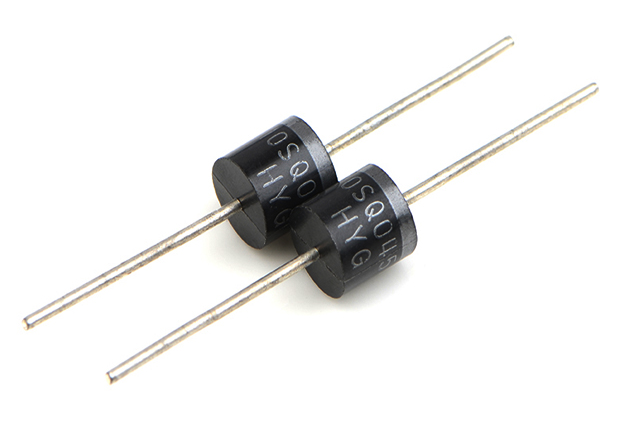
\includegraphics[width=0.5\textwidth]{photo/7.png}
  \caption{Изображение диода Шоттки}
\end{figure}


\begin{figure}[H]
  \centering
  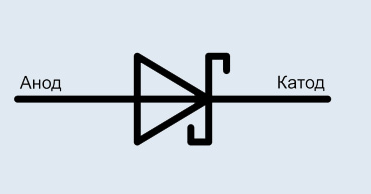
\includegraphics[width=0.5\textwidth]{photo/1.png}
  \caption{Обозначение диода Шоттки на схемах}
\end{figure}

В отличие от обычных полупроводниковых диодов, диод Шоттки известен благодаря низкому падению напряжения при его прямом включении и способностью к быстрому 
переключению. Это делает его идеальным выбором для использования в высокочастотных (ВЧ) устройствах, а также в устройствах, где используются низкие 
напряжения \cite{2}. Диод Шоттки может применяться в самых разных устройствах, например:

\begin{itemize}
  \item Для выпрямления тока большой мощности. Диоды Шоттки могут использоваться в мощных устройствах благодаря низкому падению напряжения при прямом
  включении. Эти диоды затрачивают меньше энергии, что способствует уменьшению размеров радиатора;
  \item В универсальных источниках питания. Диоды Шоттки также могут помогать разделять питание при использовании
  блоков двойного электропитания, использующих энергию электрической сети и аккумуляторов;
  \item В элементах солнечных батарей. Диоды Шоттки могут помочь добиться максимальной эффективности элементов солнечной батареи благодаря
  низкому падению напряжения при прямом включении. Также они помогают защищать ячейки от обратного заряда;
  \item В качестве защелки. Диоды Шоттки могут также использоваться в качестве защелки в транзисторных схемах, а также в цепях с
  логическими элементами 74LS или 74S.
\end{itemize}

\section{Принцип работы диодов Шоттки}

В обычном диоде полупроводники p-типа и n-типа образуют p-n-переход. В диоде Шоттки вместо полупроводника p-типа используется металл. 
Этот металл может быть разным – от платины до вольфрама, молибден, золото и т. д. 

Металл и полупроводник n-типа образуют переход металл-полупроводник. Он называется барьером Шоттки. 
Свойства барьера Шоттки различны при отсутствии напряжения смещения, при прямом и при обратном смещении.

\begin{figure}[H]
  \centering
  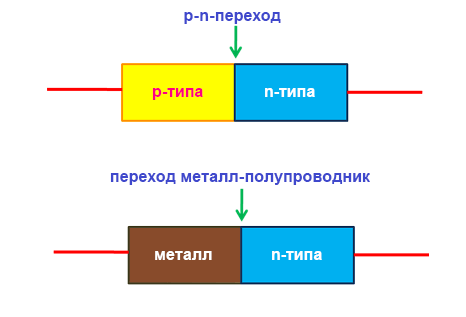
\includegraphics[width=0.5\textwidth]{photo/2.png}
  \caption{Различие между p-n переходом и переходом металла-полупроводника}
\end{figure}

\subsection{Отсутствие напряжения смещения}

При отсутствии напряжения смещения свободные электроны будут перемещаться из полупроводника n-типа в металл, чтобы восстановить равновесие.
Этот поток электронов создает барьер Шоттки, где встречаются отрицательные и положительные ионы. Чтобы свободные электроны смогли преодолеть 
этот барьер, требуется приложение внешнего напряжения большего, чем потенциал поля перехода металл-полупроводник \cite{2}.

\begin{figure}[H]
  \centering
  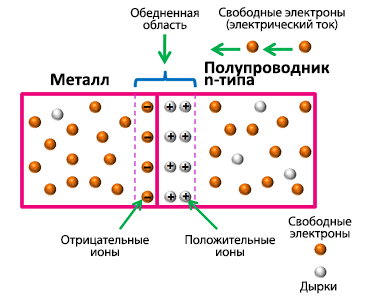
\includegraphics[width=0.5\textwidth]{photo/3.png}
  \caption{Принцип работы диода Шоттки}
\end{figure}

\subsection{Прямое смещение}

Если положительную клемму батарейки подключить к выводу диода, подключенного к металлической части перехода метал-полупроводник, а
отрицательную – к выводу диода, подключенного к полупроводнику, то таким образом мы подадим на диод прямое смещение. В этом состоянии, 
если напряжение больше 0,2 В, то электроны могут преодолеть переход металл-полупроводник и перейти из полупроводника n-типа в металл \cite{2}. 
Это приведет к возникновению тока через диод. Так работают все диоды.

\begin{figure}[H]
  \centering
  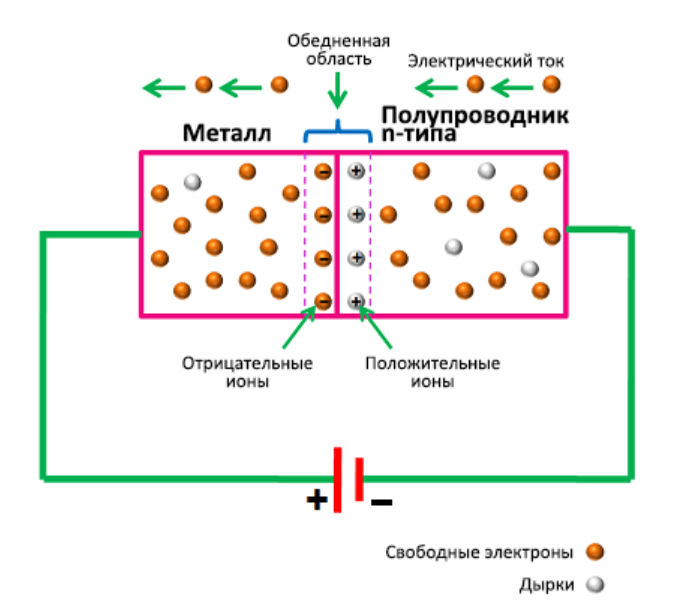
\includegraphics[width=0.5\textwidth]{photo/4.png}
  \caption{Диод Шоттки с прямым смещением}
\end{figure}

\subsection{Обратное смещение}

Если отрицательную клемму батарейки подключить к выводу диода, подключенного к металлической части перехода метал-полупроводник, 
а положительную – к выводу диода, подключенного к полупроводнику, то таким образом мы подадим на диод обратное смещение. Так мы 
увеличим ширину барьера Шоттки, не давая току течь через диод. Тем не менее, если напряжение обратного смещения будет возрастать, 
то, в конце концов, барьер будет пробит. После чего ток потечет в обратном направлении и может повредить этот и другие электронные компоненты \cite{2}.

\begin{figure}[H]
  \centering
  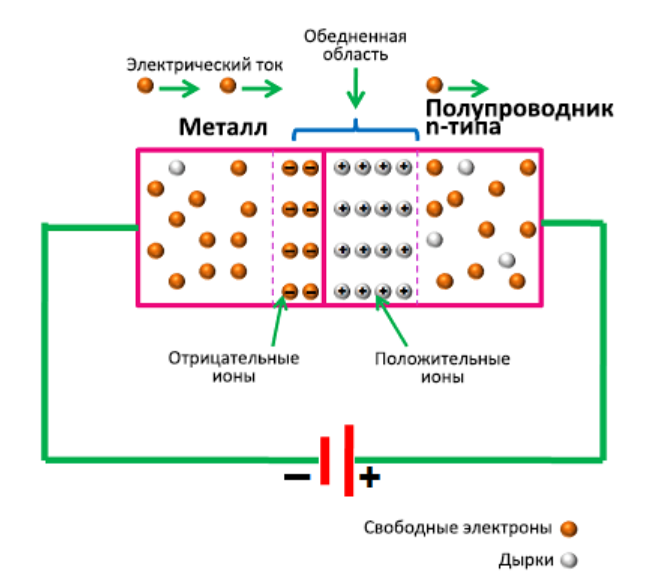
\includegraphics[width=0.5\textwidth]{photo/5.png}
  \caption{Диод Шоттки с обратным смещением}
\end{figure}

\section{Преимущества и недостатки диодов Шоттки}

Одним из главных преимуществ использования диода Шоттки вместо обычного диода является низкое сопротивление его перехода металл-полупроводник, 
приводящее к тому, что напряжение падает при его прямом включении. Таким образом диод Шоттки потребляет меньшее напряжение, чем обычный диод. 
На его p-n-переходе падает лишь 0,3-0,4 В. На рисунке 6 иожно заметить прямое падение напряжение, составляющее приблизительно 0,3 В. Ток 
через диод Шоттки значительно возрастает при увеличении напряжения сверх указанного. Через обычный диод ток не растет до напряжения приблизительно 0,6 В \cite{2}.

\begin{figure}[H]
  \centering
  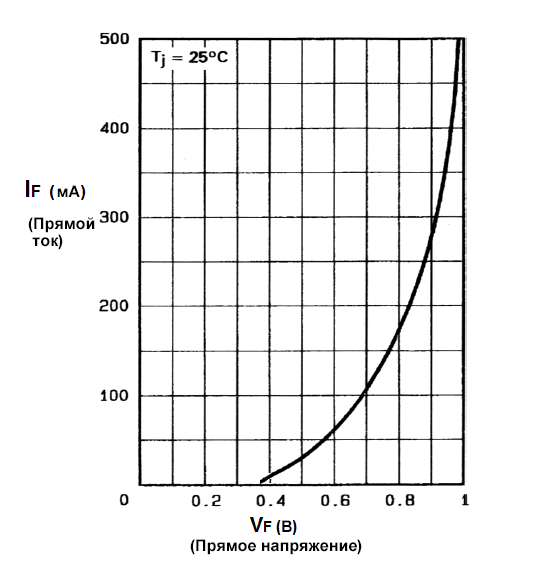
\includegraphics[width=0.5\textwidth]{photo/6.png}
  \caption{График зависимости прямого напряжения от прямого тока}
\end{figure}



Другие преимущества использования диода Шоттки вместо обычного диода:

\begin{itemize}
  \item Малое время обратного восстановления. Диод Шоттки накапливает небольшой заряд, что делает его идеальным для использования в схемах, 
  требующих быстрого переключения - они широко используются при конструировании высокочастотных печатных плат;
  \item Пониженный уровень помех. Диод Шоттки добавляет в схему меньшее количество нежелательного шума по сравнению с типичным диодом с p-n-переходом;
  \item Более высокие характеристики. Диод Шоттки потребляет меньше энергии, поэтому подходит по техническим требованиям для использования в низковольтных устройствах.
\end{itemize}


Также следует помнить о нескольких недостатках диодов Шоттки. Диод Шоттки, на который подано обратное напряжение смещения, будет пропускать больший 
обратный ток, чем обычный диод \cite{3}. Это приводит к тому, что в цепи с обратным включением диода Шоттки ток утечки больше.
 

Максимальное обратное напряжение диода Шоттки также меньше, чем у обычных диодов, и обычно составляет не более 50 В. При превышении этого напряжения 
происходит пробой диода Шоттки, в результате чего он начинает пропускать большой ток в обратном направлении. До этой величины обратного напряжения существует
лишь небольшой ток утечки через диод Шоттки, впрочем, как и у других диодов \cite{3}.


\conclusion

Таким образом, в данной работе были рассмотрены особенности, применения, преимущества и недостатки диодов Шоттки. Стоит отметить, что из-за своих достаточно
многих преимуществ спрос на диоды Шоттки велик. Их можно обнаружить в приёмниках альфа и бета излучения, детекторах нейтронного излучения, 
а в последнее время на барьерных переходах Шоттки собирают панели солнечных батарей. Так, что они питают электроэнергией и космические аппараты. Поэтому не стоит
недооценивать данный вид диодов.


\begin{thebibliography}{3}
  \bibitem{1}
  Статья <<Обозначение, применение и параметры диодов Шоттки>> [Электронный ресурс] / URL: https://go-radio.ru/diod-schottky.html (дата обращения 15.04.2022), яз. рус.
  \bibitem{2}
  Статья <<Как работают диоды Шоттки>> [Электронный ресурс] / URL: https://www.ct-electronics.ru/post/kak-rabotayet-diody-shottka (дата обращения 15.04.2022), яз. рус.
  \bibitem{3}
  Статья <<Диод Шоттки>> [Электронный ресурс] / URL: https://www.ruselectronic.com/schottky-diode/ (дата обращения 15.04.2022), яз. рус.
\end{thebibliography}


\end{document}